\section{固有振動モードの変動に関する方程式}

\begin{figure}[ht]
	\begin{center}
		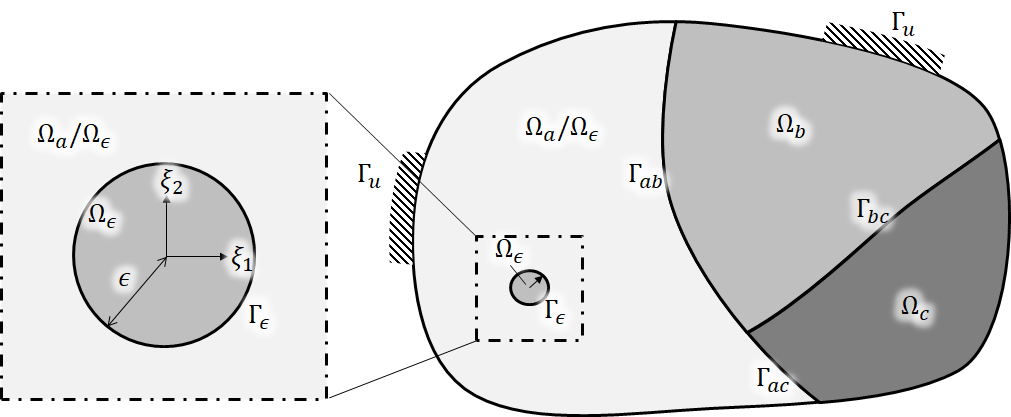
\includegraphics[width=13cm]{./figures/TD.png}
		\caption{Topological derivative}
		\label{fig:TD}
	\end{center}
\end{figure}

固有振動モードの変動$\hat{\bm{w}}(\bm{\xi})$に関する支配方程式は以下のようになる.
\begin{align}
	C_{ijkl}^{b} \hat{w}^{(-)}_{k,lj}(\bm{\xi})
	+\epsilon^2\Bigl\{(\lambda+\hat{\lambda})\rho^{b} \hat{w}_{i}^{(-)}(\bm{\xi})\Bigr\}=0
	\hspace{4.0cm}\text{in}\hspace{0.3cm}\Omega_{\epsilon}
	\label{eq:GovDisturIn}
	\\
	C_{ijkl}^{a}\hat{w}^{(+)}_{k,lj}(\bm{\xi})
	+\epsilon^2\Bigl \{\lambda\rho^{a} \hat{w}_{i}^{(+)}(\bm{\xi})
	+\hat{\lambda}\rho^{a} \Bigl(u_{i}^{}(\bm{x})+\hat{w}_{i}^{(+)}(\bm{\xi}) \Bigr) \Bigr \}=0
	\hspace{0.5cm}\text{in}\hspace{0.3cm}\Omega_{a}\backslash\Omega_{\epsilon}
	\label{eq:GovDisturOut}
	\\
	\hat{w}_{i}^{(-)}(\bm{\xi})-\hat{w}_{i}^{(+)}(\bm{\xi})=u_{i}(\bm{x})=u_{i}(\bm{x_0})+\epsilon \xi_j u_{i,j}(\bm{x_0})+O(\epsilon^2)
	\hspace{0.9cm}\text{on}\hspace{0.3cm}\Gamma_{\epsilon}
	\label{eq:GovDisturUBC}
	\\
	C_{ijkl}^{b}\hat{w}_{k,l}^{(-)}(\bm{\xi})n_{j}^{(-)}
	-C_{ijkl}^{a}\hat{w}_{k,l}^{(+)}(\bm{\xi})n_{j}^{(-)}
	=\epsilon C_{ijkl}^{a}u_{k,l}(\bm{x_0})n_{j}^{(-)}+O(\epsilon^2)
	\hspace{0.9cm}\text{on}\hspace{0.3cm}\Gamma_{\epsilon}
	\label{eq:GovDisturSBC}
	\\
	\sum_{p=1}^{n}\int_{\Omega_p}\rho^{p}(2u_{i}\hat{w}_{i}^{(+)}+\hat{w}_{i}^{(+)}\hat{w}_{i}^{(+)}) d\Omega
	+\int_{\Omega_{\epsilon}}\{\rho^{b}\hat{w}_{i}^{(-)}\hat{w}_{i}^{(-)}-\rho^{a}u_{i}u_{i}\} d\Omega=0
	\hspace{1.5cm}
	\label{eq:GovDisturNorm}
	\\
	\hat{w}_{i}^{(+)}(\bm{\xi})\rightarrow 0 \hspace{0.3cm} (|\bm{\xi}|\rightarrow \infty)
	\hspace{4.5cm}
	\label{eq:GovDisturInftyBC}
\end{align}

$\epsilon$の0次の項を整理すると
\begin{align}
	C_{ijkl}^{b} \hat{w}^{(I-)}_{k,lj}(\bm{\xi})=0
	\hspace{1.7cm}\text{in}\hspace{0.3cm}\Omega_{\epsilon}
	\label{eq:GovDisturIn1}
	\\
	C_{ijkl}^{a} \hat{w}^{(I+)}_{k,lj}(\bm{\xi})=0
	\hspace{1.2cm}\text{in}\hspace{0.3cm}\Omega\backslash\Omega_{\epsilon}
	\label{eq:GovDisturOut1}
	\\
	\hat{w}_{i}^{(I-)}(\bm{\xi})-\hat{w}_{i}^{(I+)}(\bm{\xi})=u_{i}(\bm{x_0})
	\hspace{0.7cm}\text{on}\hspace{0.3cm}\Gamma_{\epsilon}
	\label{eq:GovDisturUBC1}
	\\
	C_{ijkl}^{b}\hat{w}_{k,l}^{(I-)}(\bm{\xi})n_{j}^{(-)}
	-C_{ijkl}^{a}\hat{w}_{k,l}^{(I+)}(\bm{\xi})n_{j}^{(-)}=0
	\hspace{1.5cm}\text{on}\hspace{0.3cm}\Gamma_{\epsilon}
	\label{eq:GovDisturSBC1}
	\\
	\hat{w}_{i}^{(I+)}(\bm{\xi})\rightarrow 0\hspace{0.3cm} (|\bm{\xi}|\rightarrow \infty)
	\hspace{2.0cm}
	\label{eq:GovDisturInftyBC1}
\end{align}

$\epsilon$の1次の項を整理すると
\begin{align}
	C_{ijkl}^{b} \hat{w}^{(I\hspace{-.15em}I-)}_{k,lj}(\bm{\xi})=0
	\hspace{2.5cm}
	\text{in}\hspace{0.3cm}\Omega_{\epsilon}
	\label{eq:GovDisturIn2}
	\\
	C_{ijkl}^{a} \hat{w}^{(I\hspace{-.15em}I+)}_{k,lj}(\bm{\xi})=0
	\hspace{2.0cm}
	\text{in}\hspace{0.3cm}\Omega\backslash\Omega_{\epsilon}
	\label{eq:GovDisturOut2}
	\\
	\hat{w}_{i}^{(I\hspace{-.15em}I-)}(\bm{\xi})
	-\hat{w}_{i}^{(I\hspace{-.15em}I+)}(\bm{\xi})= \xi_j u_{i,j}(\bm{x_0})
	\hspace{2.0cm}
	\nonumber
	\\
	\equiv u_{i}^{(I\hspace{-.15em}I)}
	\hspace{1.9cm}\text{on}\hspace{0.3cm}\Gamma_{\epsilon}
	\label{eq:GovDisturUBC2}
	\\
	C_{ijkl}^{b}\hat{w}_{k,l}^{(I\hspace{-.15em}I-)}(\bm{\xi})n_{j}^{(-)}
	-C_{ijkl}^{a}\hat{w}_{k,l}^{(I\hspace{-.15em}I+)}(\bm{\xi})n_{j}^{(-)}
	=C_{ijkl}^{a} u_{k,l}^{}(\bm{x_0})n_{j}^{(-)}
	\hspace{1.0cm}
	\nonumber
	\\
	\equiv t_{i}^{(I\hspace{-.15em}I)}
	\hspace{2.0cm}\text{on}\hspace{0.3cm}\Gamma_{\epsilon}
	\label{eq:GovDisturSBC2}
	\\
	\hat{w}_{i}^{(I\hspace{-.15em}I+)}(\bm{\xi})\rightarrow 0 \hspace{0.3cm} (|\bm{\xi}|\rightarrow \infty)
	\hspace{3.0cm}
	\label{eq:GovDisturInftyBC2}
\end{align}
以上から,$\hat{\bm{w}}^{(I-)}$,$\hat{\bm{w}}^{(I+)}$,$\hat{\bm{w}}^{(I\hspace{-.15em}I-)}$,$\hat{\bm{w}}^{(I\hspace{-.15em}I+)}$は,それぞれ平衡方程式に従うことが分かる.

\newpage
